\section{Données Expérimentales}

Nous allons maintenant tester notre régulateur PID sur la plateforme afin de comparer son comportement en 
simulation à son comportement réel. Nous avons donc mis en place 4 scénarios qui permettront de comparer 
tous les cas de figure : 
\begin{enumerate}
	\item Le $1^{er}$ scénario permet de tester le fonctionnement du régulateur en boucle ouverte (mode manuel) sans FeedForward en observant sa réponse à un step de $10\%$ sur $DV$.
	\begin{python*}
		SPPath = {0: PV0} 
		ManPath = {0: True, TSim: True} # Mode manuel actif toute la simulation
		MVManPath = {0: MV0, TSim: MV0} # MV manuel reste constant
		DVPath = {0: DV0, 1300: DV0 + 10} # Step de 10% après 1300 secondes
		FF = False # Pas de FeedForward
		ManFF = False # Pas de prise en compte du FeedForward 
	\end{python*}
	\item Le $2^{ème}$ scénario permet de de tester le fonctionnement du régulateur en boucle ouverte et avec FeedForward en observant 
	sa réponse à un step de $10\%$ sur $DV$.
	\begin{python*}
		SPPath = {0: PV0}
		ManPath = {0: True, TSim: True} #Mode manuel actif toute la simulation
		MVManPath = {0: MV0, TSim: MV0} # MV manuel reste constant
		DVPath = {0: DV0, 1300: DV0 + 10} # Step de 10% après 1300 secondes
		FF = True # FeedForward activé
		ManFF = True # Prise en compte du FeedForward
	\end{python*}
	\item Le $3^{ème}$ scénario permet de tester le fonctionnement du régulateur en boucle fermée (mode automatique) sans FeedForward en observant sa réponse
	à un step de $-10\%$ sur $SP$ puis un step de $10\%$ sur $DV$.
	\begin{python*}
		SPPath = {0: PV0 + 5, 1000: PV0 - 5} # Step de -10% après 1000 secondes
		ManPath = {0: True, 500: False, TSim: False} 
		MVManPath = {0: MV0+15, TSim: MV0+15}
		DVPath = {0: DV0, 1600: DV0 + 10} # Step de 10% après 1600 secondes
		FF = False # Pas de FeedForward
		ManFF = False 
	\end{python*}
	\item Le $4^{ème}$ scénario permet de compléter le scnéario précédant en testant le fonctionnement du régulateur en boucle fermée FeedForward en observant sa réponse à un step
	de $-10\%$ sur $SP$ puis à un step de $10\%$ sur $DV$.
	\begin{python*}
		SPPath = {0: PV0 + 5, 1000: PV0 - 5} #Step de -10% après 1000 secondes
		ManPath = {0: True, 500: False, TSim: False} # Mode automatique après 500 secondes
		MVManPath = {0: MV0+15, TSim: MV0+15} 
		DVPath = {0: DV0, 1600: DV0 + 10} # Step de 10% après 1600 secondes
		FF = True # FeedForward activé
		ManFF = False 
	\end{python*}
\end{enumerate}

\subsection{Scénario 1}
\begin{figure}[H]
	\centering
	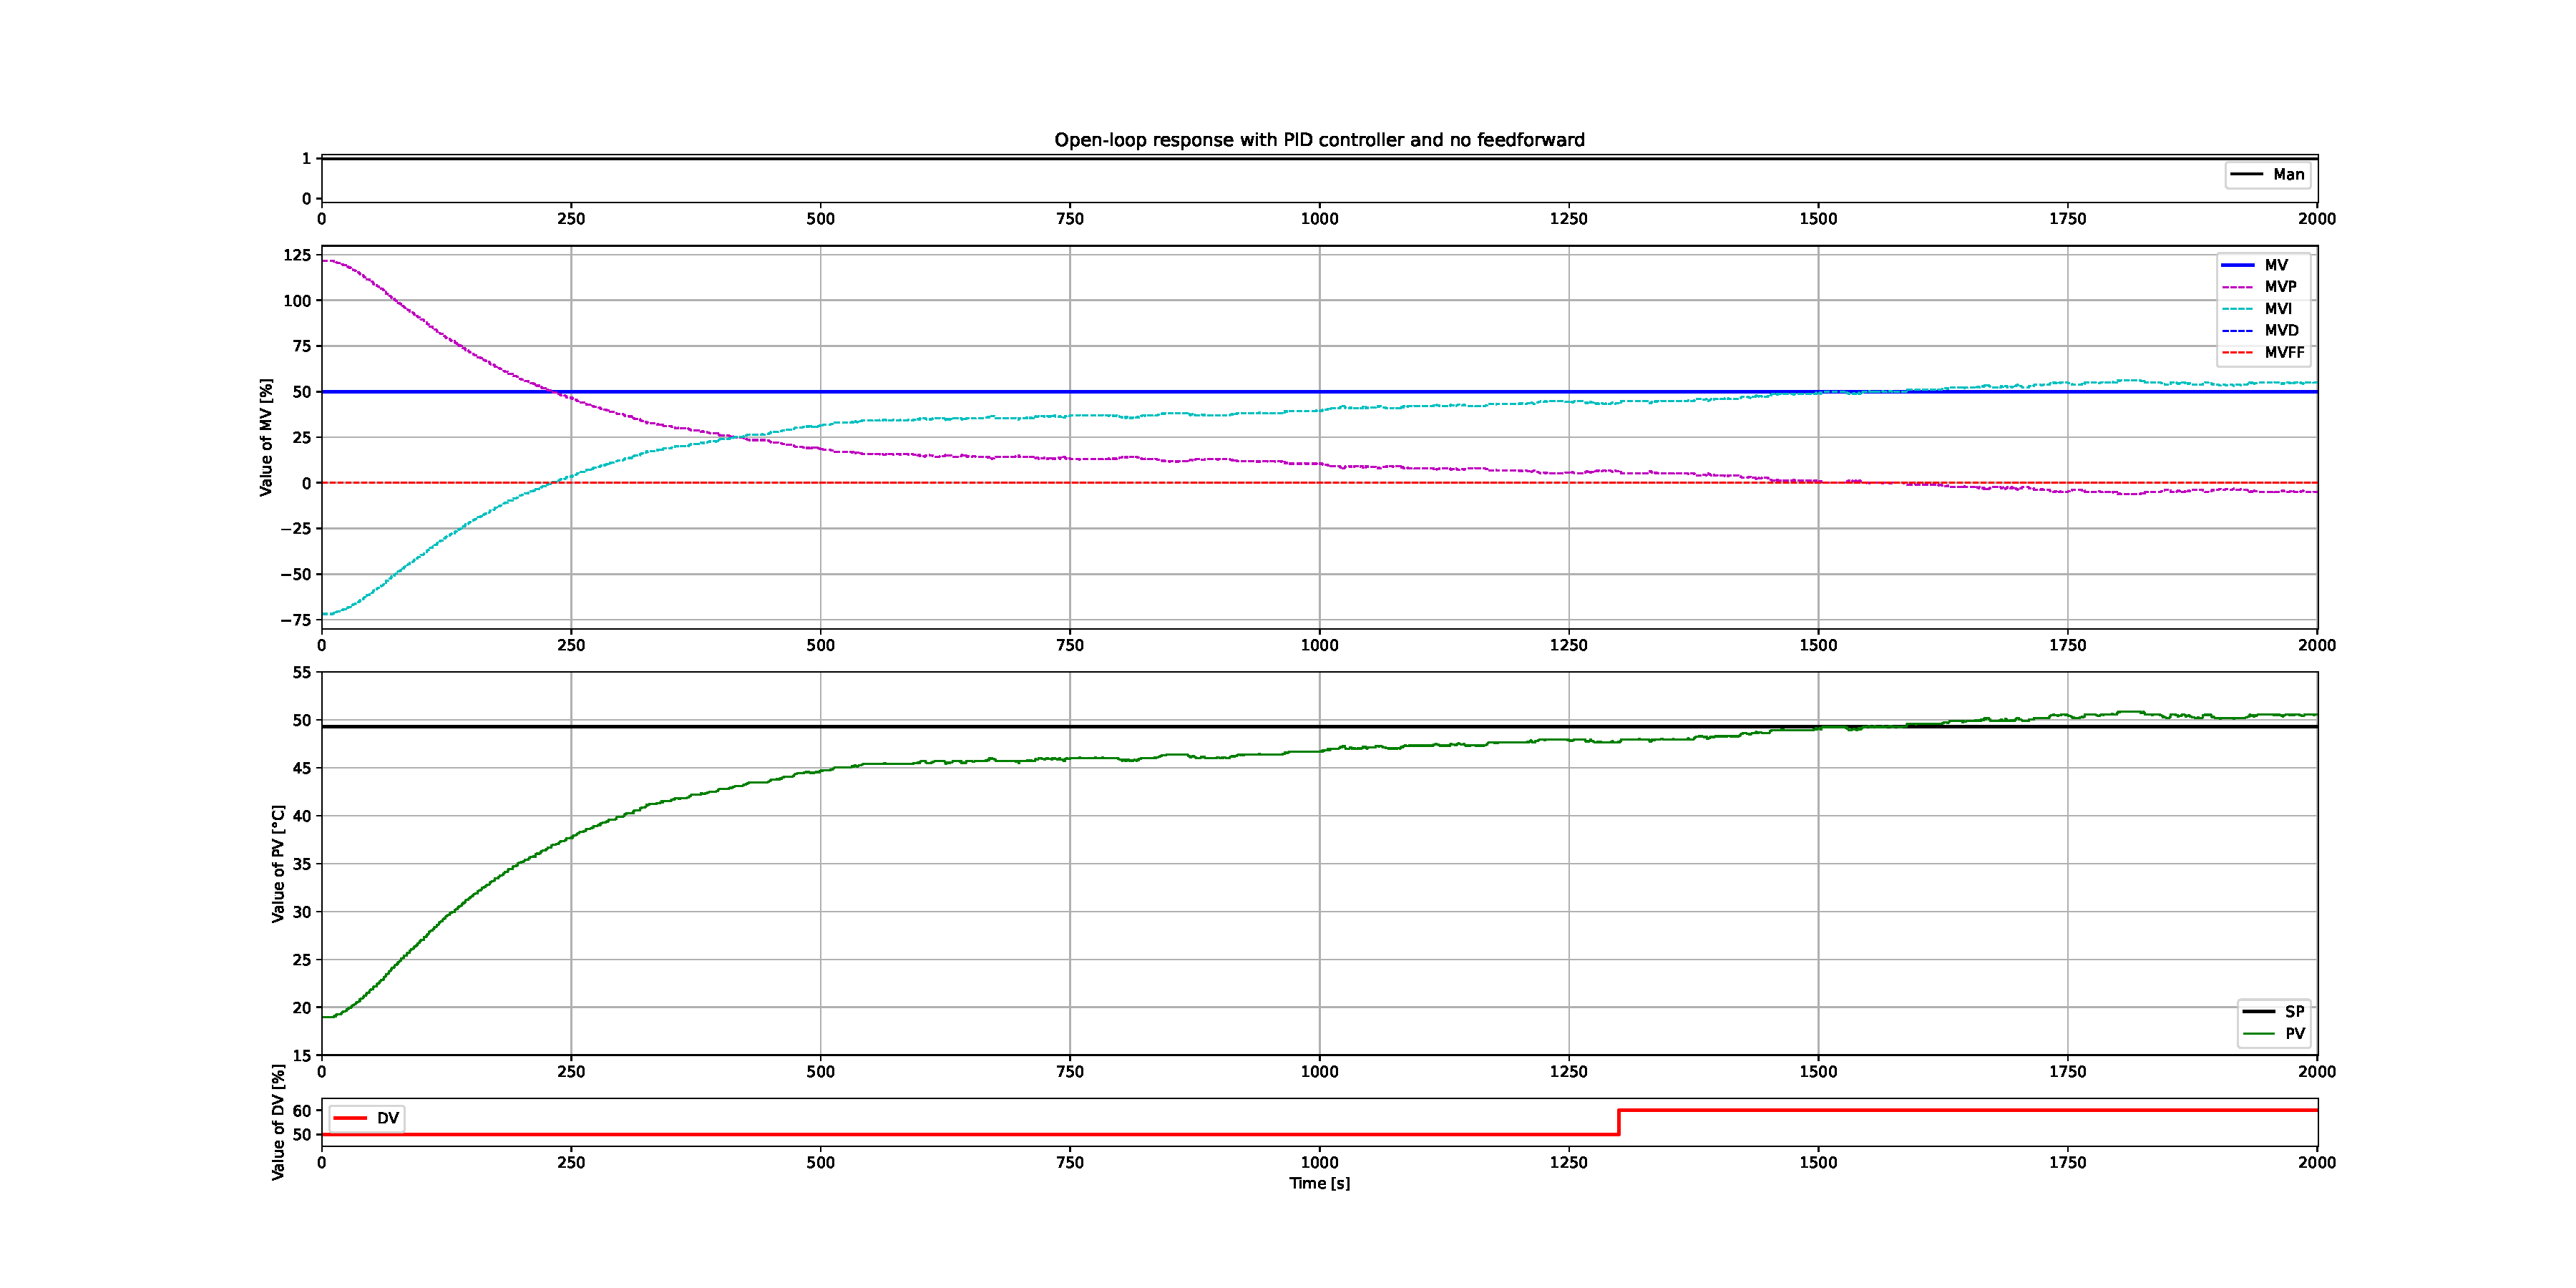
\includegraphics[width=1\textwidth]{../Plots/Experiment_scenario_2_2024-03-30-20h20.pdf}
	\caption{Données expérimentales du $1^{er}$ scénario}
	\label{fig:exp_scenario1}
\end{figure}
\begin{figure}[H]
	\centering
	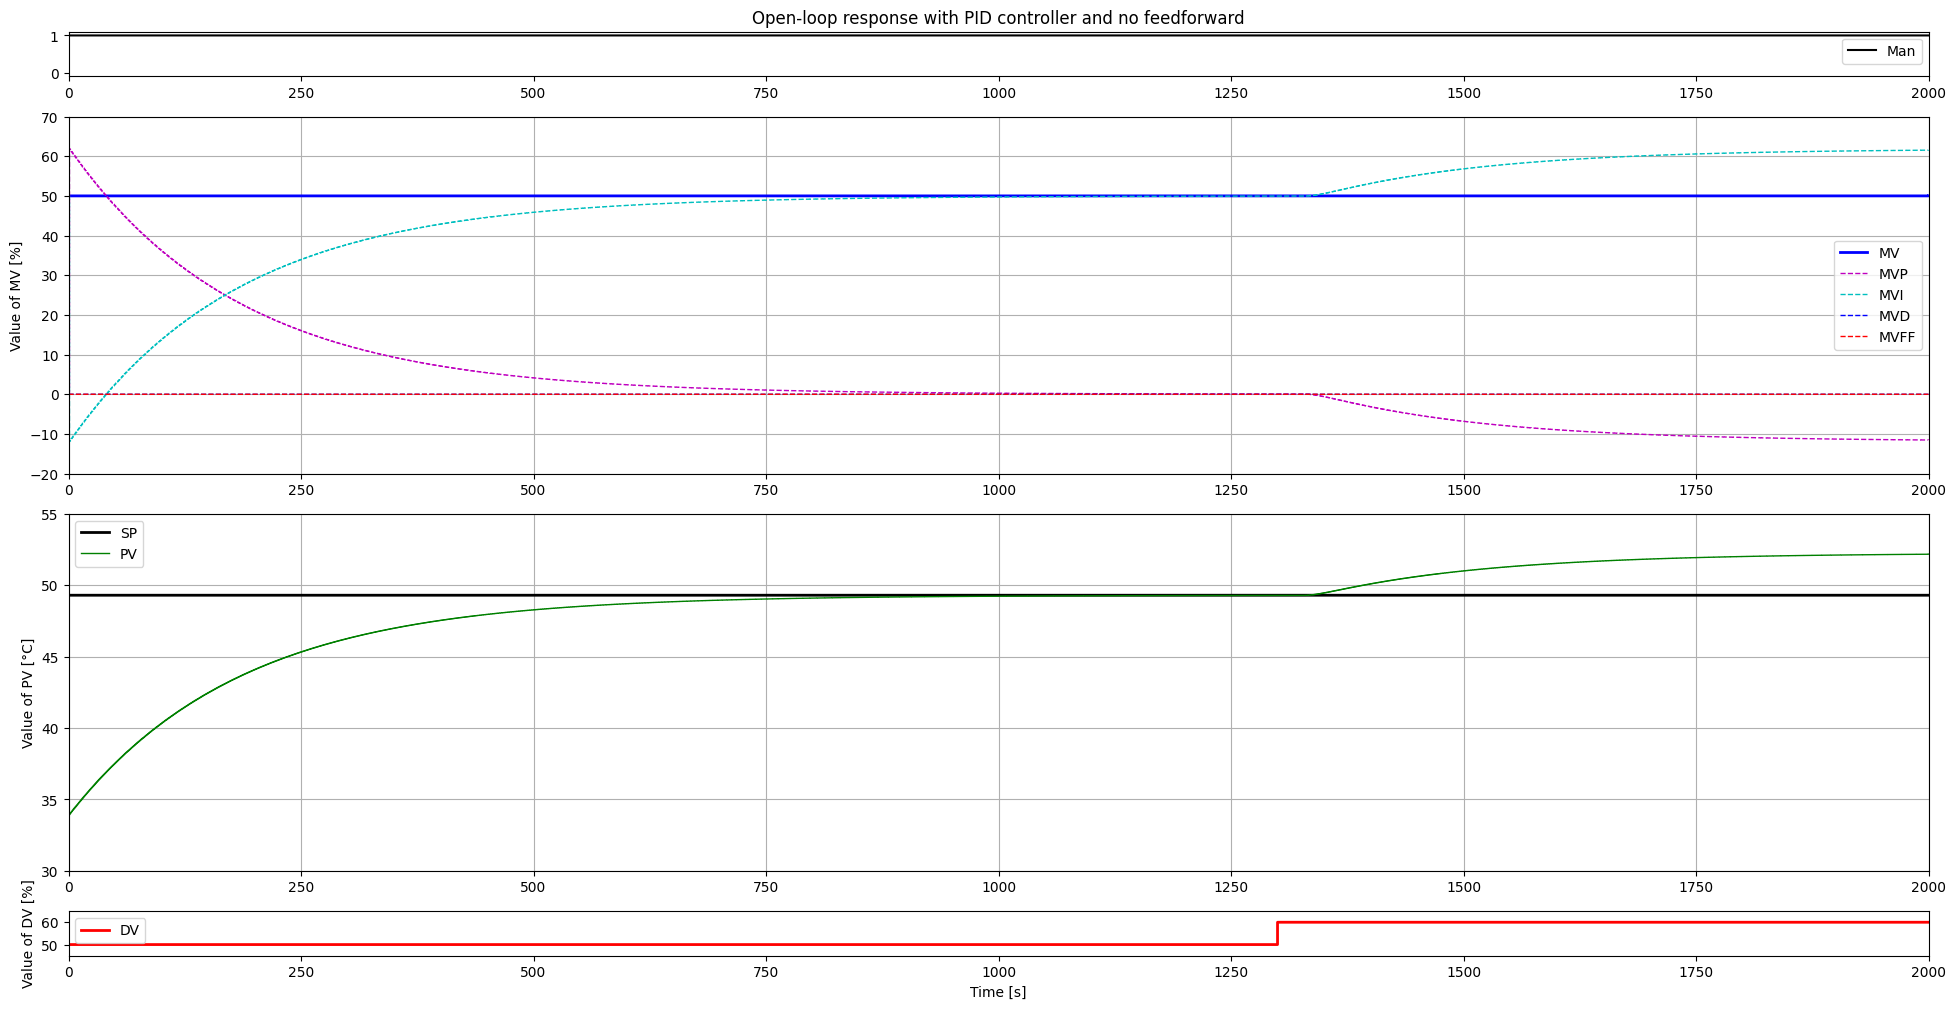
\includegraphics[width=0.8\textwidth]{figures/scenario2.png}
	\caption{Données de la simulation du $1^{er}$ scénario}
	\label{fig:sim_scenario1}
\end{figure}

On peut observer que le $PV$ n'a pas atteint la valeur de consigne ($SP$) avant le step de $10\%$ sur $DV$. Cela est dû au fait que, pour l'expérience,
la valeur du $PV$ à $t = 0s$ est de $\sim 18\degree C$ tandis que pour la simulation, il est de $\sim 34\degree C$. Néanmoins, une fois le step de $10\%$ sur $DV$ effectué,
la valeur du $PV$ converge jusqu'à la valeur de consigne et la dépasse à $t = 1500s$ ce qui correspond à un retard par rapport à la simulation $\sim \Delta t = 75s$. 
\\Une autre observation importante concerne la forme de la courbe $PV$ qui suggère un comportement typique d'un système du second ordre. Cependant, l'analyse des dynamiques du système 
avait révélé une seconde constante de temps très faible, $T_2P \sim 10^{-12}$, négligeable, ce qui a conduit à la conclusion que notre système se comportait
plutôt comme un système du premiere ordre en réponse à un changement sur $MV$. Selon nous, une des causes serait la température plus basse de la pièce qui affecterait 
l'inertie thermique du capteur de température. L'humidité de la pièce pourrait aussi être facteur puisque celle-ci affecte la conductivité thermique de l'air 
ambiant et donc pourrait aussi impacter l'inertie thermique du capteur.

\subsection{Scénario 2}

\begin{figure}[H]
	\centering
	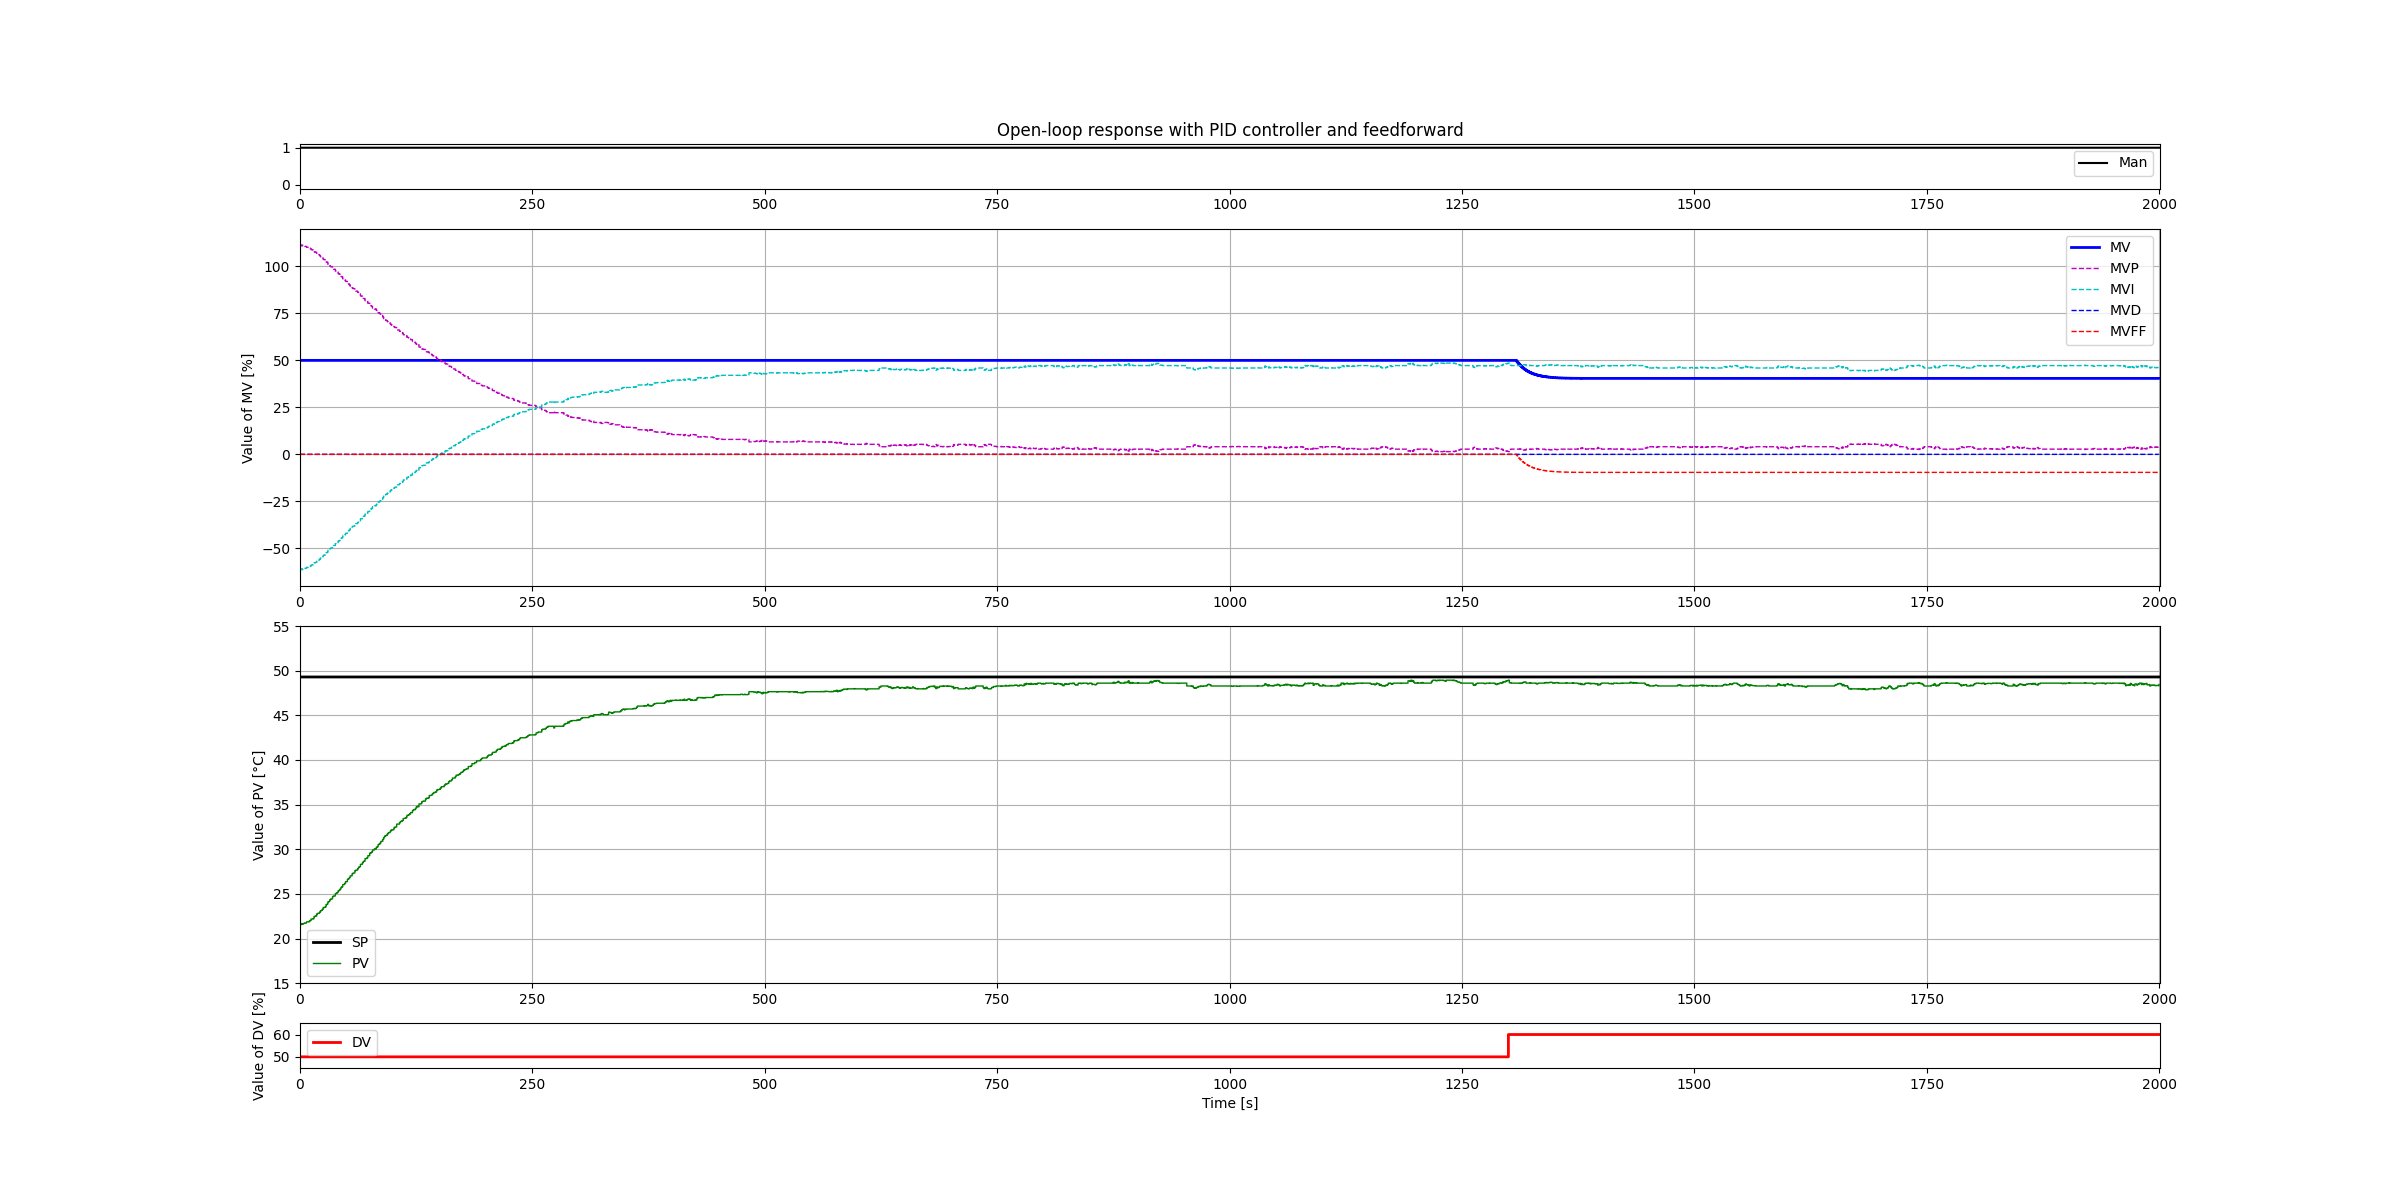
\includegraphics[width=1\textwidth]{../Plots/Experiment_scenario_3_2024-03-30-19h18.png}
	\caption{Données expérimentales du $2^{ème}$ scénario}
	\label{fig:exp_scenario2}
\end{figure}
\begin{figure}[H]
	\centering
	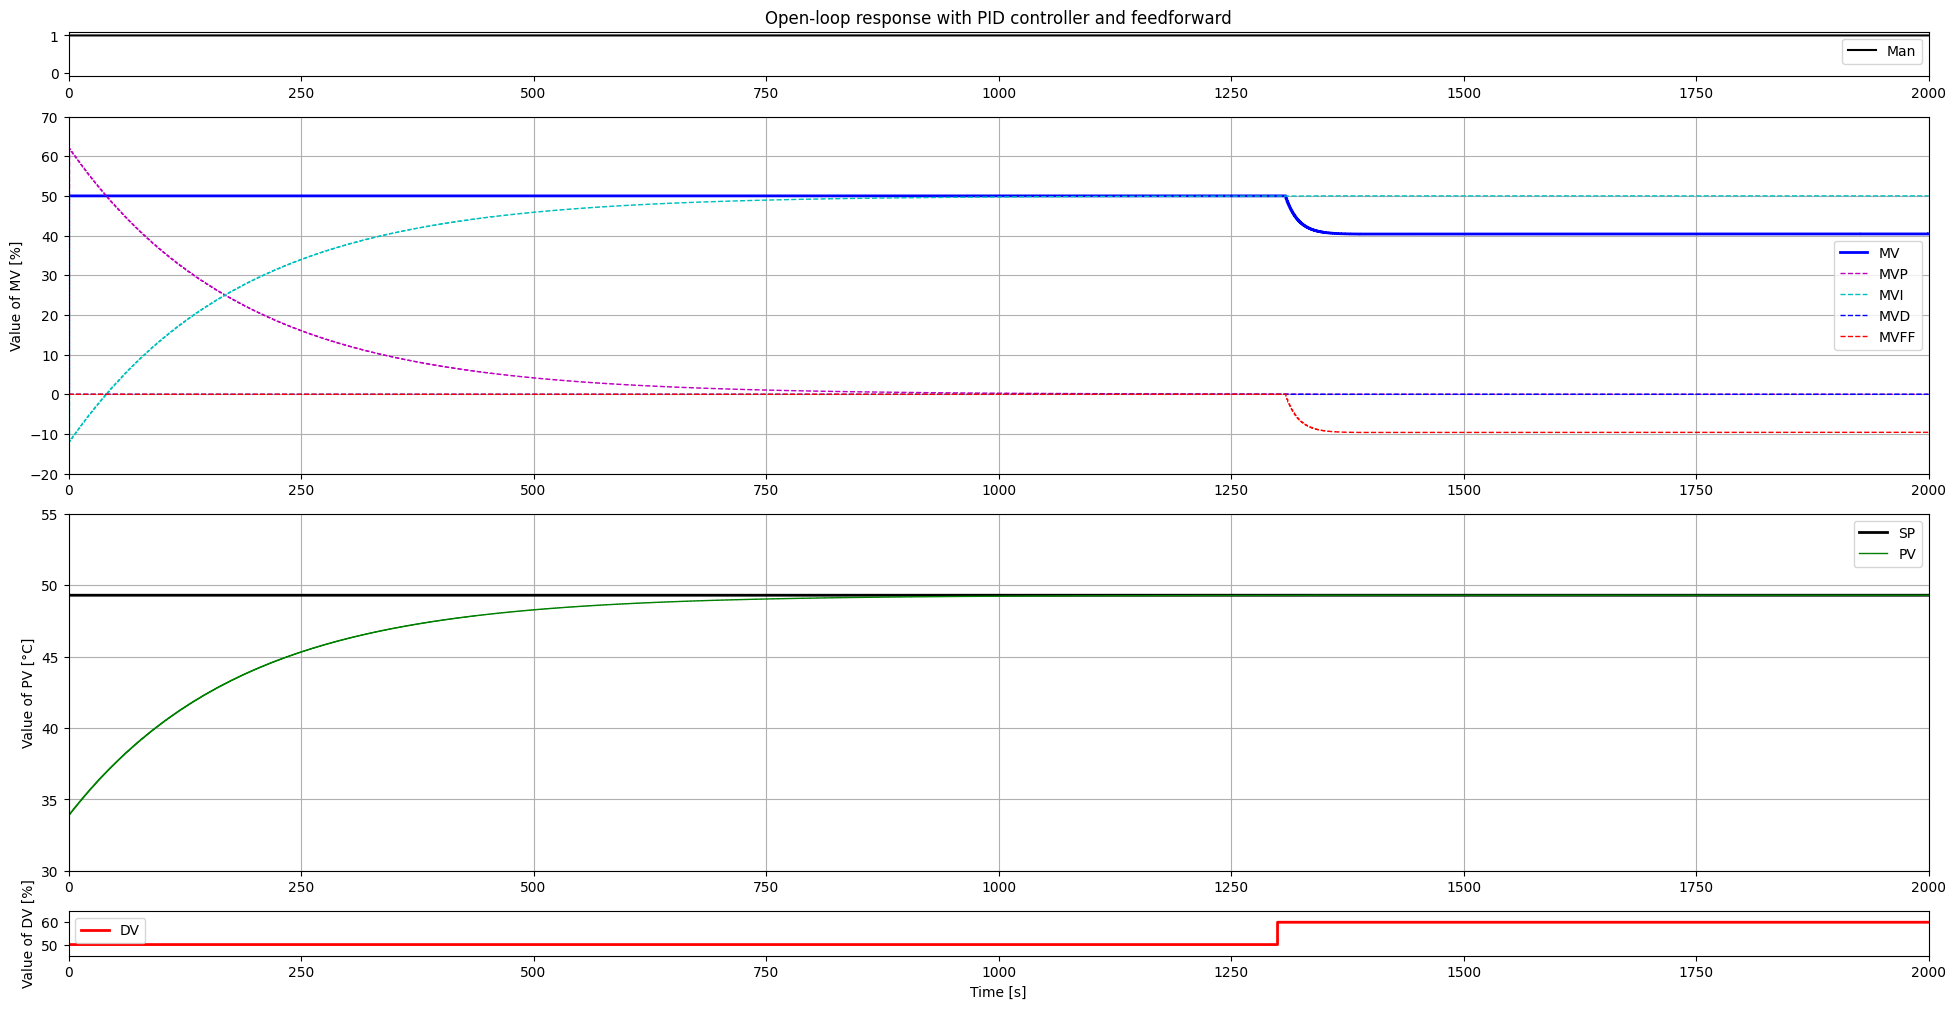
\includegraphics[width=0.8\textwidth]{figures/scenario3.png}
	\caption{Données de la simulation du $2^{ème}$ scénario}
	\label{fig:sim_scenario2}
\end{figure}

Comme pour le scénario précédent(\ref{fig:exp_scenario1}), on peut voir que le système régit plutôt comme un système du second ordre.
\\Cependant, contrairement à l'exemple précédent, la valeur du $PV$ atteint à peu près au même moment la valeur de consigne ($SP$) que pour la simulation. Ceci est dû au fait
que la température du capteur n'a pas suffisamment pu redescendre entre les deux scénarios. En effet, la valeur de $PV$ à $t = 0s$ est de $\sim 22\degree C$ ce qui correspond 
à $4\degree C$ de plus que pour le scénario précédent. 
\\\`A part cela, le système réagit bien à la perturbation grâce au FeedForward qui permet de compenser entièrement le step de $10\%$ sur $DV$.

\subsection{Scénario 3}

\begin{figure}[H]
	\centering
	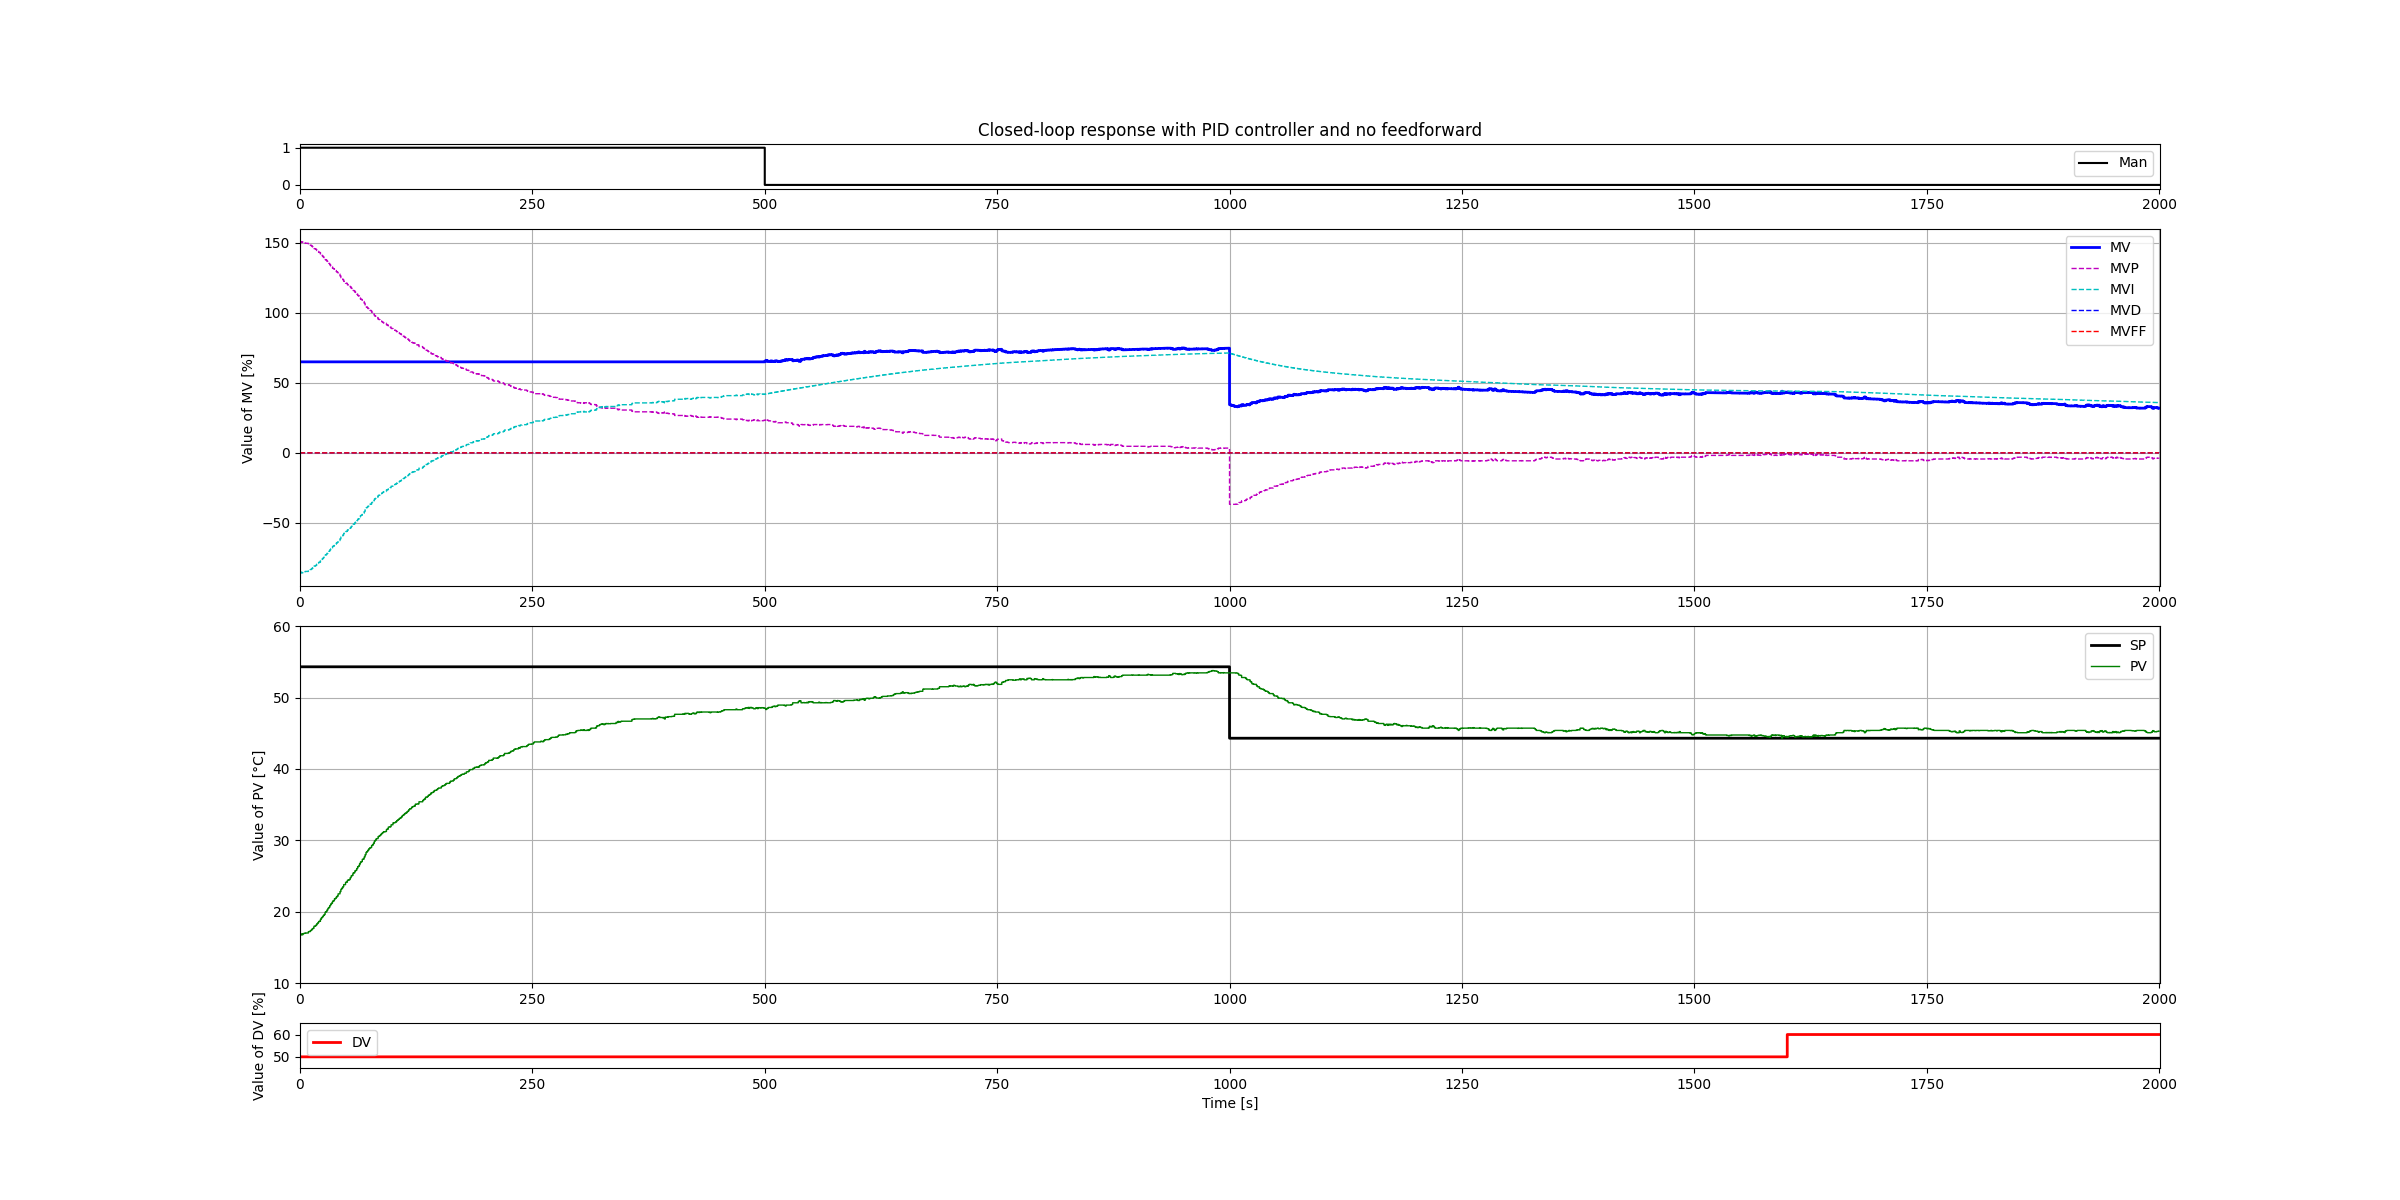
\includegraphics[width=1\textwidth]{../Plots/Experiment_scenario_5_2024-03-30-15h32.png}
	\caption{Données expérimentales du $3^{ème}$ scénario}
	\label{fig:exp_scenario3}
\end{figure}
\begin{figure}[H]
	\centering
	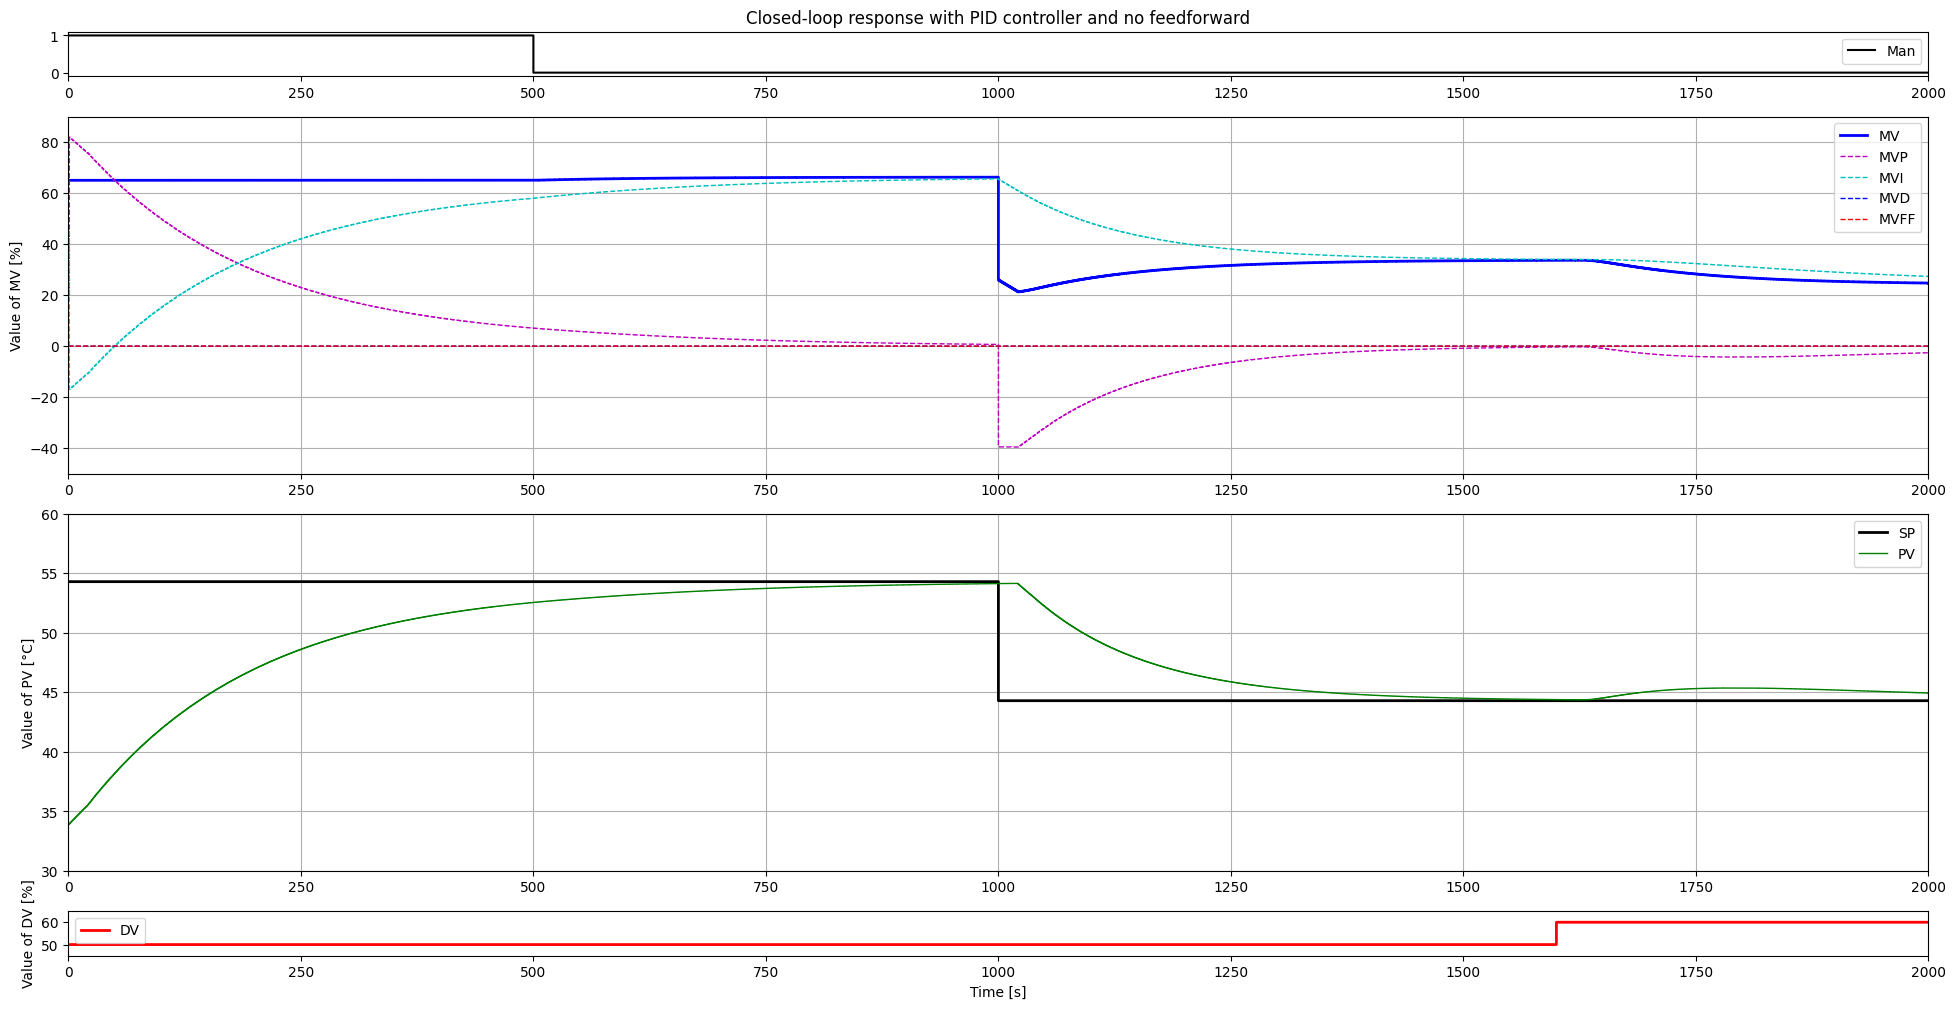
\includegraphics[width=0.8\textwidth]{figures/scenario5.png}
	\caption{Données de la simulation du $3^{ème}$ scénario}
	\label{fig:sim_scenario3}
\end{figure}

